\chapter{Introduzione}
La teoria dell'informazione si occupa di studiare la trasmissione di informazione da una sorgente ad un destinatario, tramite un canale.
Sebbene a prima vista sembra si tratti di una applicazione molto specifica, in realtà la teoria dell'informazione ha importanti 
conseguenze (ed applicazioni) in moltissimi settori.

Il ``padre'' della teoria dell'informazione è Claude Shannon, che nel 1948 nel celebre articolo ``Mathematical Theory of Communication'' formulò i concetti chiave della teoria, come quello di entropia. Seguirono poi altri importanti risultati (molti dei 
quali sempre ad opera di Shannon).

La teoria di Shannon è una teoria matematica ed astratta, nella quale i dettagli tecnici (come il mezzo fisico che costituisce il canale) non hanno nessuna importanza. Questa assunzione consente quindi di applicare la teoria in svariate situazioni.

Il sistema di comunicazione di base preso in esame da Shannon è rappresentato in figura \ref{fig:0005}.
Esso è costituito da:
\begin{enumerate}
\item sorgente: entità che genera l'informazione
\item canale: mezzo attraverso il quale l'informazione si propaga
\item destinatario: entità che riceve l'informazione
\end{enumerate}

\begin{figure}[htbp]
\begin{center}
	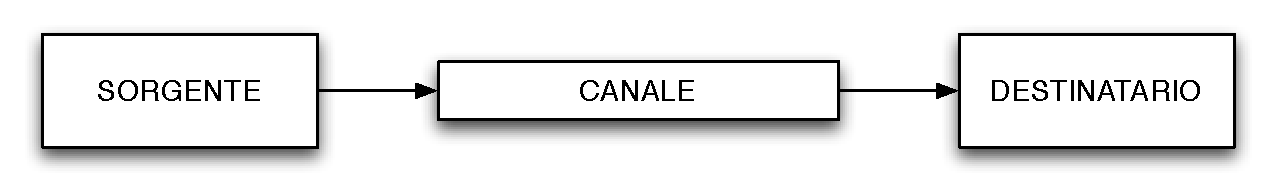
\includegraphics[width=0.9\textwidth]{img/intro1.pdf}
\caption{sistema di comunicazione di base per la teoria di Shannon}
\label{fig:0005}
\end{center}
\end{figure}

Il sistema appena presentato è minimale, nel senso che contiene unicamente le componenti necessarie ad instaurare 
la comunicazione. Una situazione più realistica è quella presentata in figura \ref{fig:0006}. In questo caso sono presenti 
due blocchi aggiuntivi: un sistema di codifica e un sistema di decodifica.
E' infatti in generale necessario codificare i dati da trasmettere a seconda del canale di comunicazione (ad opera della sorgente) e decodificarli una volta ricevuti (da parte del destinatario).

\begin{figure}[htbp]
\begin{center}
	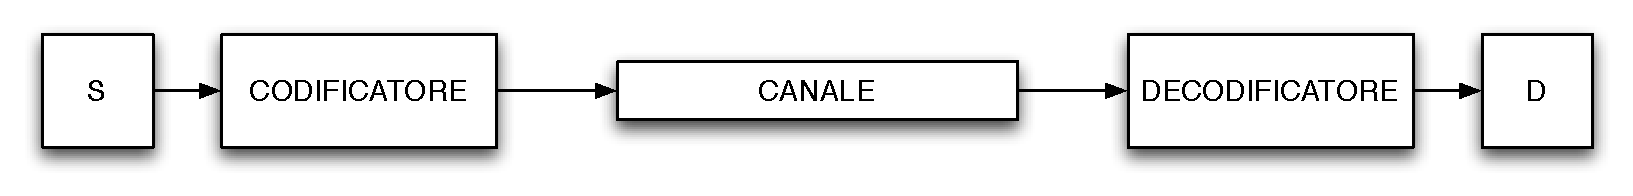
\includegraphics[width=\textwidth]{img/intro2.pdf}
\caption{sistema di comunicazione dotato di codificatore e decodificatore}
\label{fig:0006}
\end{center}
\end{figure}

Ponendosi in un caso ancora più generale, è necessario considerare anche la presenza del rumore. Tipicamente infatti non è possibile 
avere un canale di comunicazione \emph{affidabile}. A causa di molti fattori (e.g. interferenze) sarà infatti possibile che ciò che 
viene inviato dalla sorgente non coincida con quanto ricevuto dal destinatario. Quest'ultimo scenario è rappresentato in figura 
\ref{fig:0007}.

\begin{figure}[htbp]
\begin{center}
	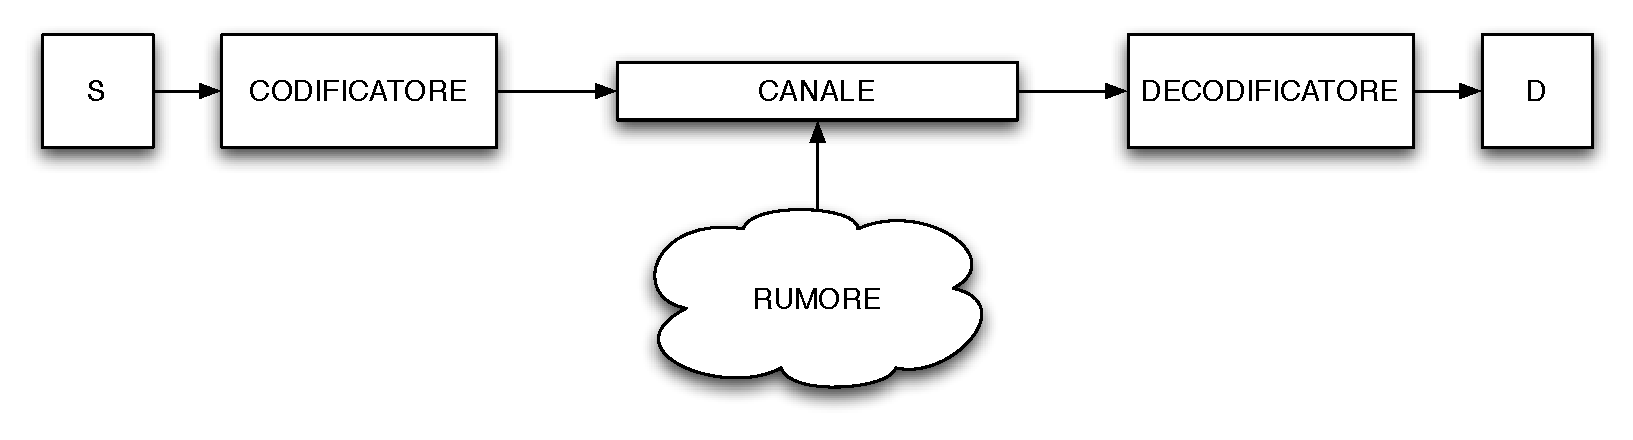
\includegraphics[width=\textwidth]{img/intro3.pdf}
\caption{sistema di comunicazione dotato di codificatore e decodificatore, con presenza di rumore}
\label{fig:0007}
\end{center}
\end{figure}

La teoria dell'informazione si occupa dunque di problemi che coinvolgono la trasmissione di informazione da un luogo a un altro, o da un tempo ad un altro (ad esempio la memorizzazione di file in un hard disk per una successiva lettura). In questo ultimo caso 
sorgente e destinazione coincidono.
I problemi di base da affrontare sono due:
\begin{enumerate}
\item \textbf{efficienza}: Migliorare l'efficienza della trasmissione, riducendo la quantità di informazione inviata.
In questo modo è possibile aumentare la velocità di trasmissione (o ridurre le dimensioni da memorizzare nell'esempio dell'hard disk).
\item \textbf{affidabilità}: Rendere la comunicazione affidabile nel caso del rumore, introducendo quindi dell'informazione aggiuntiva 
che consenta di ricostruire l'informazione originale, anche in presenza di errori.
\end{enumerate}

I due problemi sono collegati da un concetto chiave, che è quello di \textbf{ridondanza}. In generale infatti per aumentare l'efficienza si cercherà di eliminare l'informazione ``inutile'', riducendo il messaggio al minimo necessario per renderlo comprensibile. Per aumentare invece l'affidabilità sarà necessario aggiungere informazione, in maniera da poter individuare e correggere eventuali errori 
in fase di trasmissione.
Si tratta dunque di due problemi chiaramente in contrasto.

\noindent
Alcune osservazioni:
\begin{enumerate}
\item il canale considerato è unidirezionale: nei contesti reali i canali sono invece spesso bidirezionali. Possiamo però pensare semplicemente a due canali differenti con uno scambio di ruoli tra l'entità sorgente e l'entità destinatario
\item la sorgente e il destinatario sono unici, mentre nella realtà possono esserci n sorgenti e m destinatari, collegati con k canali, con flussi bidirezionali (pensiamo ai sistemi multimediali); questo fa parte dell'area della teoria dell'informazione che si occupa del broadcasting (diffusione delle informazioni) che non saranno considerate.
\end{enumerate}


Facciamo ora un esempio concreto: in figura \ref{fig:bsc} è rappresentato un \textbf{Binary Symmetric Channel (BSC)}.
\begin{figure}[htbp]
\begin{center}
	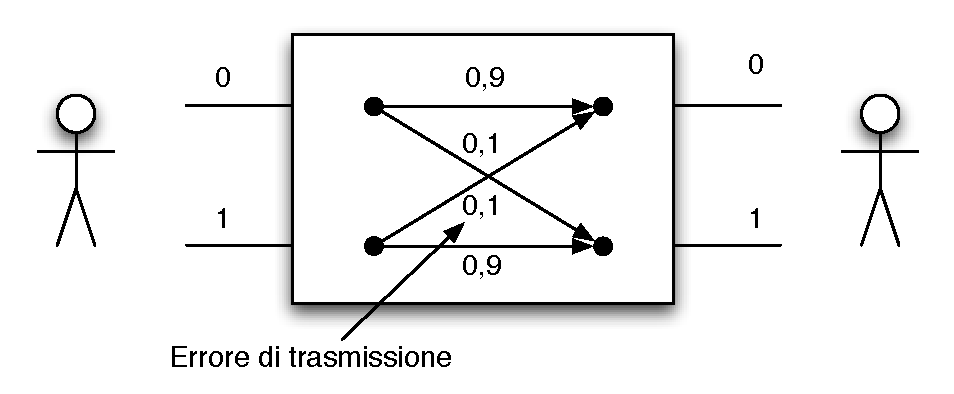
\includegraphics[width=0.7\textwidth]{img/bsc.pdf}
\caption{Binary Symmetric Channel}
\label{fig:bsc}
\end{center}
\end{figure}
Si tratta di un canale caratterizzato da due ingressi e due uscite. Supponiamo di conoscere statisticamente il canale e di aver 
compreso, dopo averlo osservato, che quando la sorgente invia 0, il destinatario riceve 0 il 90\% delle volte, mentre riceve 1 nel 10\% dei casi (c'è quindi una probabilità di errore). La stessa cosa è stata osservata anche per quel che riguarda la trasmissione di 1.
Per migliorare l'affidabilità del canale, possiamo inviare delle terne di bit. Per esempio, quando la sorgente vuole 
inviare 0 viene in realtà mandato 000, mentre quando vuole mandare 1 viene inviato 111. Il destinatario considererà come simbolo 
inviato, quello che appare più volte nel messaggio che riceve (e.g. 0 se riceve 001, 1 se riceve 111).
Con questa semplice tecnica abbiamo aumentato l'affidabilità del canale (chiaramente la probabilità di errore è più bassa), tuttavia 
ciò è avvenuto a scapito dell'efficienza. Dobbiamo infatti inviare il triplo dei simboli necessari, riducendo quindi di un fattore 3 
la velocità di trasmissione.

Sebbene sembri difficile conciliare queste due esigenze, un compromesso è rappresentato dal \textbf{secondo teorema di Shannon}, presentato alla fine della dispensa. Si tratta di un teorema non costruttivo: Shannon non fornisce il codice in questione, ma fornisce una dimostrazione sull'assurdità della non esistenza di tale codice, che ad oggi comunque non è stato ancora trovato (ci si è però avvicinati molto con i turbo-code).

\noindent
Definiamo ora in maniera più formale alcuni concetti.

\begin{definizione}[sorgente]
Si dice \textit{sorgente} un insieme di simboli \(\{s_1, s_2 ... s_n\}\).
\end{definizione}

\noindent
Conosciamo la sorgente quando conosciamo la probabilità con cui viene emesso ciascun simbolo.

\noindent
Possiamo distinguere tra:
\begin{enumerate}
\item \textbf{sorgenti discrete}: se possono generare un numero finito di simboli (quelle che prenderemo in esame)
\item \textbf{sorgenti continue}: se possono generare un numero infinito di simboli
\end{enumerate}

\noindent
Un'ulteriore distinzione è fra:
\begin{enumerate}
\item \textbf{sorgenti a memoria zero}: in cui l'emissione dei simboli è indipendente dai simboli generati in precedenza
\item \textbf{sorgenti con memoria}: quelle che troviamo tipicamente nel mondo reale, caratterizzate da una certa dipendenza della generazione dei simboli rispetto ai precedenti
\end{enumerate}

Nel nostro caso il concetto di sorgente coincide con il concetto di variabile aleatoria. C'è infatti una una corrispondenza perfetta tra i due: la sorgente emette simboli casuali caratterizzati ognuno da una probabilità di essere generato.

Supponiamo quindi che X sia una variabile aleatoria il cui dominio è \(\X = \{x_1, x_2 ... x_n\}\) caratterizzata da una distribuzione di probabilità \(p(x) = Pr\{X = x\}\), con \(x \in \X\).

Il problema che ci poniamo è quello di stabilire quanto sia informativa la sorgente: per far questo dobbiamo innanzitutto stabilire cosa si intende per informazione. L'informazione può essere considerata a 3 diversi livelli di crescente complessità:
\begin{enumerate}
\item \textbf{simbolico} (o sintattico): riguarda i singoli simboli e il modo in cui interagiscono tra loro, i vincoli di varia natura, non si preoccupa del significato;
\item \textbf{semantico}: riguarda ciò che la sorgente vuol dire al destinatario a livello di significato, si tratta di un'astrazione del modello della frase;
\item \textbf{pragmatico}: si distingue dalla semantica per ciò che la sorgente vuole intendere (ad esempio, se considero il messaggio ``Sai che ora è?'', non voglio una risposta sì/no, ma l'ora, ed è qui che entra in gioco la pragmatica, che riguarda ciò che voglio dire).
\end{enumerate}

\noindent
La teoria dell'informazione di Shannon si occupa dell'informazione a livello simbolico.

\medskip
\noindent
La dispensa è articolata in tre parti:
\begin{enumerate}
\item \textbf{formalizzazione della teoria dell'informazione}: in cui saranno date le definizioni di entropia e gli altri concetti chiave della teoria dell'informazione
\item \textbf{problemi di trasmissione in assenza di rumore}: dove ci si concentrerà sull'efficienza (ignorando il rumore), cercando quindi di eliminare la ridondanza
\item \textbf{problemi di trasmissione in presenza di rumore}: in cui si concentrerà sulla realizzazione di una trasmissione affidabile, cercando di conciliare efficienza e affidabilità
\end{enumerate}